\documentclass[10pt,a4paper]{article}
\usepackage[utf8]{inputenc}
\usepackage{amsmath}
\usepackage{amsfonts}
\usepackage{amssymb}
\usepackage{graphicx}
\usepackage{kotex}
\usepackage{hyperref}
\usepackage{listings}
\usepackage[super]{nth}
\usepackage[english]{babel}
\graphicspath{{../}}

%% Page Layout %%
\usepackage[left=2.5cm,right=2.5cm,top=3cm,bottom=3cm,a4paper]{geometry}
\setlength{\parskip}{1.5ex}
%
% Homework Details
%   - Title
%   - Due date
%   - Class
%   - Section/Time
%   - Instructor
%   - Author
%

\newcommand{\hwTitle}{Homework Assignment\ \#1}
\newcommand{\DueDate}{March 25, 2019}
\newcommand{\Semester}{Spring 2019}
\newcommand{\Course}{CS380}
\newcommand{\CourseInstructor}{Prof. Jinah Park}
\newcommand{\AuthorName}{Inyong Koo}
\newcommand{\StudentID}{20160042}


%% Headnote, footnote %%
\usepackage{fancyhdr}
\pagestyle{fancy}

\fancyhf{}
\rhead{\StudentID \, \AuthorName}
\lhead{\Semester}
\chead{\Course \, \hwTitle}
\cfoot{\thepage}

\renewcommand{\headrulewidth}{1pt}
\renewcommand{\footrulewidth}{1pt}

\fancypagestyle{titlepagestyle}
{
	\fancyhf{}
	\rhead{Due date: \DueDate}
	\lhead{\Semester}
	\cfoot{\thepage}
	\renewcommand{\footrulewidth}{1pt}
}

\begin{document}
	\title{\vspace{-7ex}\Course \, Introduction to Computer Graphics \\ \hwTitle}
	\author{\textbf{Snowflake 2D Animation} \\\\ \StudentID \ \AuthorName}
	\date{\hrule}
	%\date{}  % Toggle commenting to test
	
	\maketitle
	
	\thispagestyle{titlepagestyle}
	
	\paragraph{}
	In this document, I will explain how my implementation (shown in \autoref{fig:execution}) satisfies the given specifications. I will not copy the code itself, but rather explain in plain text. So if you want to see how the actual implementation looks like, please refer to the code lines and comments from attached files. I'll note where to look for each task.
	
	\begin{figure}[h]
		\centering
		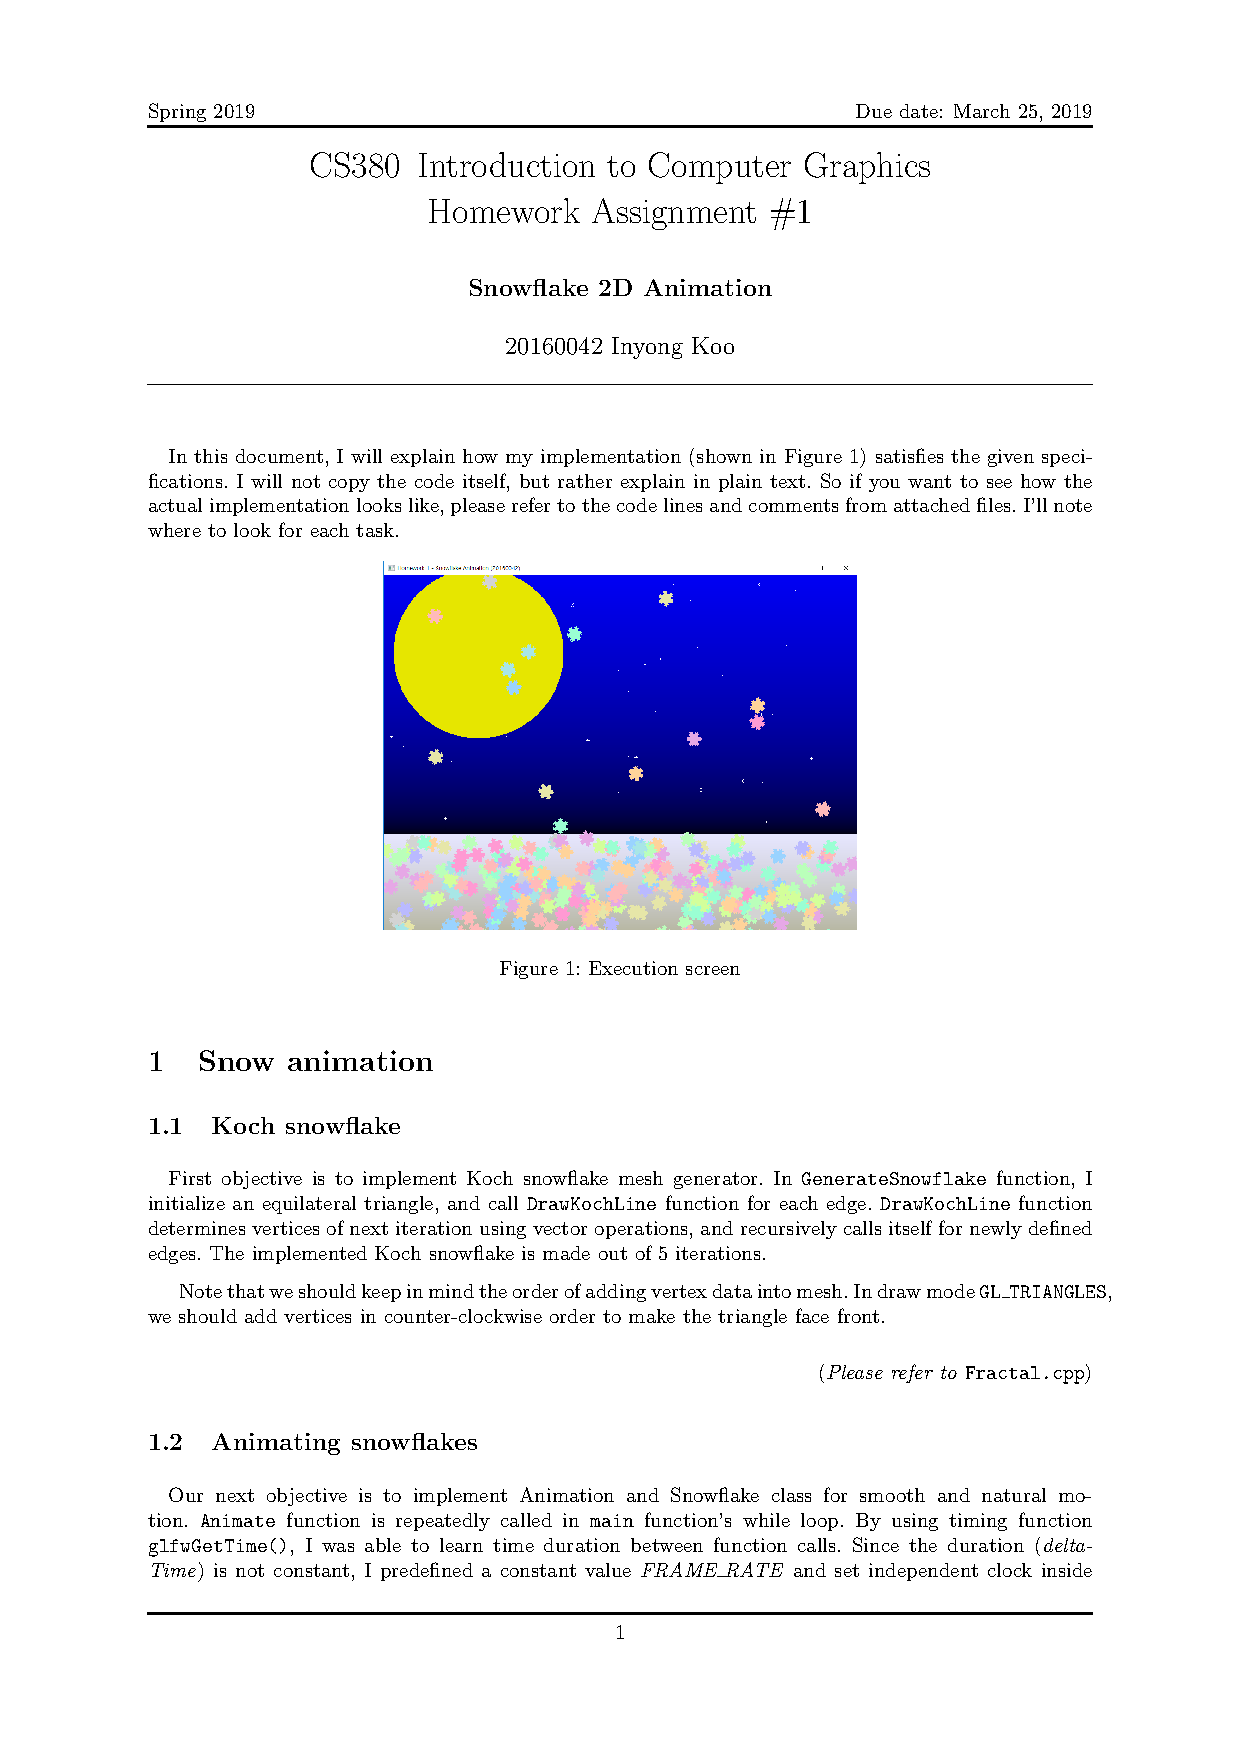
\includegraphics[width=0.5\linewidth]{HW1.png}
		\caption{Execution screen}
		\label{fig:execution}
	\end{figure}
	
	\section{Snow animation}
	
	\subsection{Koch snowflake}
	\paragraph{}
	First objective is to implement Koch snowflake mesh generator. In \texttt{GenerateSnowflake} function, I initialize an equilateral triangle, and call \texttt{DrawKochLine} function for each edge.  \texttt{DrawKochLine} function determines vertices of next iteration using vector operations, and recursively calls itself for newly defined edges. The implemented Koch snowflake is made out of 5 iterations.
	
	Note that we should keep in mind the order of adding vertex data into mesh. In draw mode \textbf{\texttt{GL\_TRIANGLES}}, we should add vertices in counter-clockwise order to make the triangle face front.

	\begin{flushright}
		(\emph{Please refer to} \texttt{Fractal.cpp})
	\end{flushright}

	\subsection{Animating snowflakes}
	\paragraph{}
	Our next objective is to implement Animation and Snowflake class for smooth and natural motion. \texttt{Animate} function is repeatedly called in \texttt{main} function's while loop. By using timing function \texttt{glfwGetTime()}, I was able to learn time duration between function calls. Since the duration (\emph{deltaTime}) is not constant, I predefined a constant value \emph{FRAME\_RATE} and set independent clock inside the \texttt{Animate} function. 'motions' are executed only if the clock value gets larger than \emph{FRAME\_RATE}, where the clock value is returns to 0. Therefore, the 'motions' are executed over same time interval. Using the same principle, a snowflake is generated outside the viewing rectangle every 0.25 second. (This happens in \texttt{main} function.)
	
	The 'motions' are defined in Snowflake class;
	\texttt{SpinSnowflake} function changes orientation of each snowflake in constant rate. \texttt{FallSnowflake} function changes position of each snowflake. A snowflake moves in constant speed towards y-axis, and randomly choose direction and amount of x-axis translation for each frame. But such implementation showed random, somewhat chaotic behavior, so I kept x-axis translation of its previous frame and applied weighted average with it to acquire smooth motion. 
			
	\texttt{CheckFallen} function determines whether the snowflake has 'fallen'. Each snowflake has random, different \textit{\_ground} value. When a snowflake reaches the \emph{\_ground}, it stops its motion and stay. However, since a snowflake is generated on every 0.25 second, keeping all those snowflake objects will cause lags, or even overflow error. So I removed the 'fallen snowflakes' when there are more than 300 snowflake objects in \emph{snowflakes} vector.
	\begin{flushright}
		(\emph{Please refer to} \texttt{Animation.cpp} \emph{and} \texttt{Snowflake.cpp})
	\end{flushright}
	
		
	\section{Background}
	\paragraph{}
	Another specification for assignment 1 is to construct a gradient background scene with two different kinds of objects with different colors. 
	
	\subsection{Gradient rectangle}
	\paragraph{}
	I draw two adjacent rectangles to depict a snowing, night scenary. blue-black gradient color was used in upper rectangle to express the night sky, and white-yellow gradient color was used in lower rectangle to express the snow covered ground illuminating yellow moonlight. The rectangles are drawn in draw mode \texttt{GL\_TRIANGLE\_STRIP}.
	
	\begin{flushright}
		(\emph{Please refer to} \texttt{GenerateGradientRectangle} \emph{function in} \texttt{main.cpp})
	\end{flushright}
	
	\subsection{Mesh 1 - Moon object}
	\paragraph{}
	I draw the moon using draw mode \texttt{GL\_TRIANGLE\_FAN}. Moon object is simply a yellow circle, where first vertex is the center, and other vertices are laid on the circle, counter-clockwise order. Since \texttt{DefaultMaterial} class sets its color white, I updated its color later using \texttt{UpdateColor} function.
	
	\begin{flushright}
		(\emph{Please refer to} \texttt{GenerateBackgroundMeshType1} \emph{function in} \texttt{main.cpp})
	\end{flushright}
	
	\subsection{Mesh 2 - Stars object}
	\paragraph{}
	I draw the stars using draw mode \texttt{GL\_LINES}. My original intention was to use \texttt{GL\_POINTS}, but our vertex shader does not handle \texttt{GL\_POINTS} and caused error while rendering. Instead, I used short lines to implement similar effect. Furthermore, I was able to differentiate stars into 3 groups; small ($ \cdot $) , middle (+), and large ($ \ast $). I randomly selected position of the stars in 'sky' region. 
	
	\begin{flushright}
		(\emph{Please refer to} \texttt{GenerateBackgroundMeshType2} \emph{function in} \texttt{main.cpp})
	\end{flushright}

	\pagebreak
	\section{Creativity}
	\paragraph{}
	20 points of this assignment's grading is 'creativity' score. It means that my animation should not only meet the specifications, but also take a step further to make it look interesting and nice. I put a lot of effort to make my 2D animation to compose a 'scenary'. (For instance, I could have just put different two colored triangles for background meshs, but instead tried to depict the night sky by implementing the moon and the stars.) In this section, I'd like to appeal some 'creative' features of my implementation.
	
	\begin{itemize}
		\item A snowflake randomly chooses its color from 13 options, and stays on the ground after it has 'fallen'. Since snowflake is '눈꽃' in korean, I thought it would be interesting to make some kind of flower bed from fallen snowflakes, rather than let them just disappear below the window. Since snowflakes are constructed on same depth (z value), I had to alter rendering order to get later snowflakes gets above the older snowflakes.
		
		\item Using random variable with weighted average on snowflake animation allowed each snowflake to have independent, smooth, and natural descending path. 
		
		\item I used background rectangle meaningfully by seperating regions - sky and ground. Snowflakes halt when they're in ground region, and stars are created only in sky region.
		
		\item I tried to differentiate not only colors of two background objects, but also their draw mode, so that I could express my understanding on different modes.
		
	\end{itemize} 
		
	
\end{document}